\hypertarget{yertle-the-turtle}{%
\section{Yertle the Turtle}\label{yertle-the-turtle}}

\begin{figure}[!ht]
  \begin{adjustwidth}{-\oddsidemargin-1in}{-\rightmargin}
    \centering
    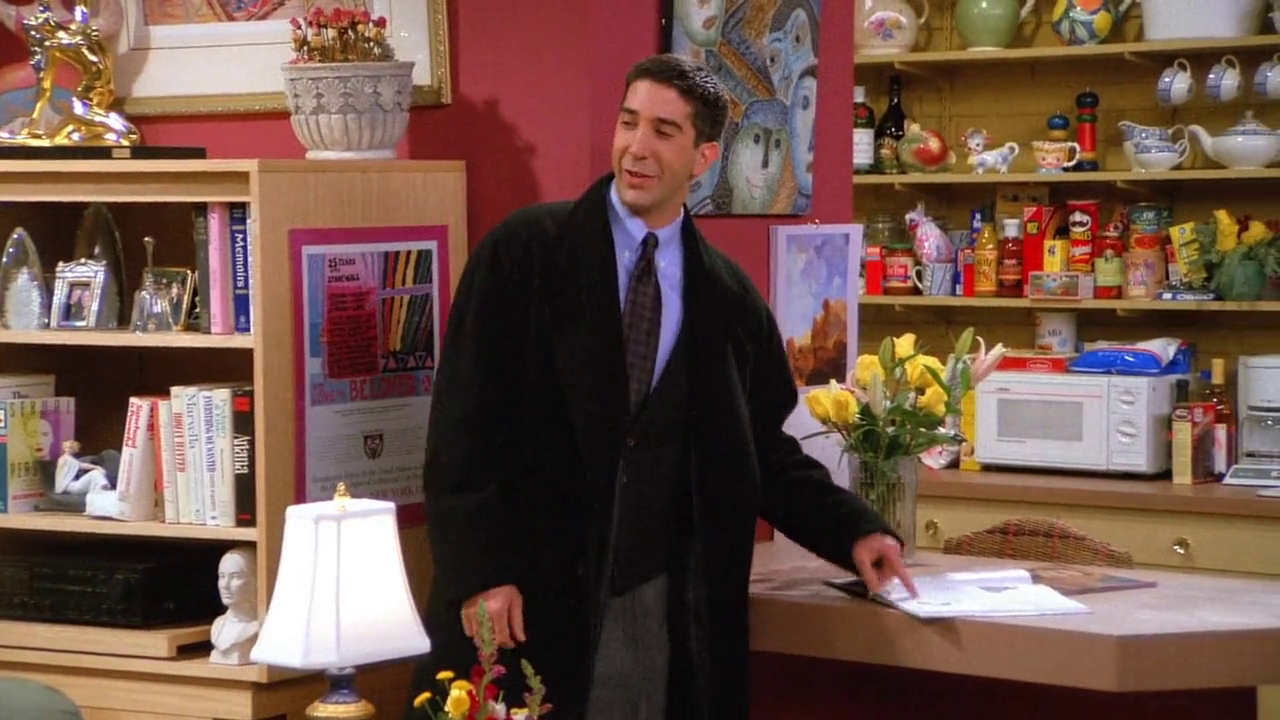
\includegraphics[trim={0 4cm 0 3cm,}, clip, width=\paperwidth]{./S01/img/9/yertle-the-turtle.png}
    \caption{Yertle the Turtle\label{fig:yertle-the-turtle}}
  \end{adjustwidth}
\end{figure}

\begin{tcolorbox}[enhanced,center upper,
    drop fuzzy shadow southeast, boxrule=0.3pt,
    lower separated=false,
    colframe=black!30!dialogoBorder,colback=white]
\begin{minipage}[c]{0.14\linewidth}
  \raisebox{\dimexpr-\height+\ht\strutbox\relax}{
    
\includegraphics[width=1.5cm]{./assets/img/ross.png}
  }
   & \centering \scriptsize{Ross}
\end{minipage}
\hspace{.1mm}
\begin{minipage}[c]{0.8\linewidth}
  \textbf{- Hey, hey, Yertle the Turtle. A classic.}\\
  - A Tartaruga Yertle. Um clássico.
\end{minipage}
\end{tcolorbox}

Quando foi buscar seu ``crânio'' que havia emprestado a Carol, Ross
notou na mesa da cozinha o livro \emph{Yertle the Turtle} (1958),
conhecido livro de fábula do \emph{Dr.~Seuss} (1904-1991), um renomado
autor infantil que criou, entre outros personagens, o \emph{Grinch}.

\begin{figure}
  \centering
  \begin{tikzpicture}
    \node [inner sep=0pt] at (0,0) {
      
\includegraphics[width=0.8\textwidth,keepaspectratio]{./S01/img/9/yertle-the-turtle-book.png}
    };
    \draw [white, rounded corners=\ClipSep, line width=\ClipSep]
    (current bounding box.north west) --
    (current bounding box.north east) --
    (current bounding box.south east) --
    (current bounding box.south west) -- cycle
    ;
    \end{tikzpicture}
    \caption{Yertle the Turtle - Livro\label{fig:yertle-the-turtle-livro}}
\end{figure}

\hypertarget{referuxeancias}{%
\subsection{Referências}\label{referuxeancias}}

\begin{itemize}
\tightlist
\item
  \sloppy Site oficial. \url{https://www.seussville.com/characters/yertle-the-turtle/}
\item
  \sloppy Fandom Wiki. \url{https://seuss.fandom.com/wiki/Yertle_the_Turtle_and_Other_Stories}
\end{itemize}

\hypertarget{macys}{%
\section{Macy's}\label{macys}}

\begin{figure}[!ht]
  \begin{adjustwidth}{-\oddsidemargin-1in}{-\rightmargin}
    \centering
    
\includegraphics[trim={0 6cm 0 2cm,}, clip, width=\paperwidth]{./S01/img/9/macys.png}
    \caption{Macy’s\label{fig:macy-s}}
  \end{adjustwidth}
\end{figure}

\begin{tcolorbox}[enhanced,center upper,
    drop fuzzy shadow southeast, boxrule=0.3pt,
    lower separated=false,
    colframe=black!30!dialogoBorder,colback=white]
\begin{minipage}[c]{0.14\linewidth}
  \raisebox{\dimexpr-\height+\ht\strutbox\relax}{
    
\includegraphics[width=1.5cm]{./assets/img/joey.png}
  }
   & \centering \scriptsize{Joey}
\end{minipage}
\hspace{.1mm}
\begin{minipage}[c]{0.8\linewidth}
  \textbf{- We used to work together.}\\
  - Nós trabalhávamos juntos.
\end{minipage}

\medskip
\begin{minipage}[c]{0.14\linewidth}
  \raisebox{\dimexpr-\height+\ht\strutbox\relax}{
    
\includegraphics[width=1.5cm]{./assets/img/obsession-girl.png}
  }
   & \centering \scriptsize{Girl}
\end{minipage}
\hspace{.1mm}
\begin{minipage}[c]{0.8\linewidth}
  \textbf{- We did?}\\
  - Trabalhamos?
\end{minipage}

\medskip
\begin{minipage}[c]{0.14\linewidth}
  \raisebox{\dimexpr-\height+\ht\strutbox\relax}{
    
\includegraphics[width=1.5cm]{./assets/img/joey.png}
  }
   & \centering \scriptsize{Joey}
\end{minipage}
\hspace{.1mm}
\begin{minipage}[c]{0.8\linewidth}
  \textbf{- Yeah, at Macy's. You're the Obsession girl, right? I was the Aramis guy.}\\
  - Na Macy's. Era a garota Obsession, certo? Eu era o cara Aramis.
\end{minipage}
\end{tcolorbox}

Num reencontro com uma conhecida de trabalho, Joey menciona que
trabalhou com ela na \emph{Macy's} (1830), conhecida loja de
departamento americana. Ele menciona \emph{Obsession} e \emph{Aramis},
ambos perfumes que podem ser comprados na loja. O movimento que ele faz
com a mão faz referência a maneira como ele oferecia uma amostra do
perfume.

Joey volta a trabalhar oferecendo amostras de perfume no episódio
\textbf{\textcolor{primarycolor}{S02E02 - Aquele do leite materno}}.

\hypertarget{referuxeancias-1}{%
\subsection{Referências}\label{referuxeancias-1}}

\begin{itemize}
\tightlist
\item
  \sloppy Site oficial (Inglês). \url{https://www.macysinc.com/about/history}
\end{itemize}

\hypertarget{dont-stand-so-close-to-me}{%
\section{Don't Stand So Close To Me}\label{dont-stand-so-close-to-me}}

\begin{figure}[!ht]
  \begin{adjustwidth}{-\oddsidemargin-1in}{-\rightmargin}
    \centering
    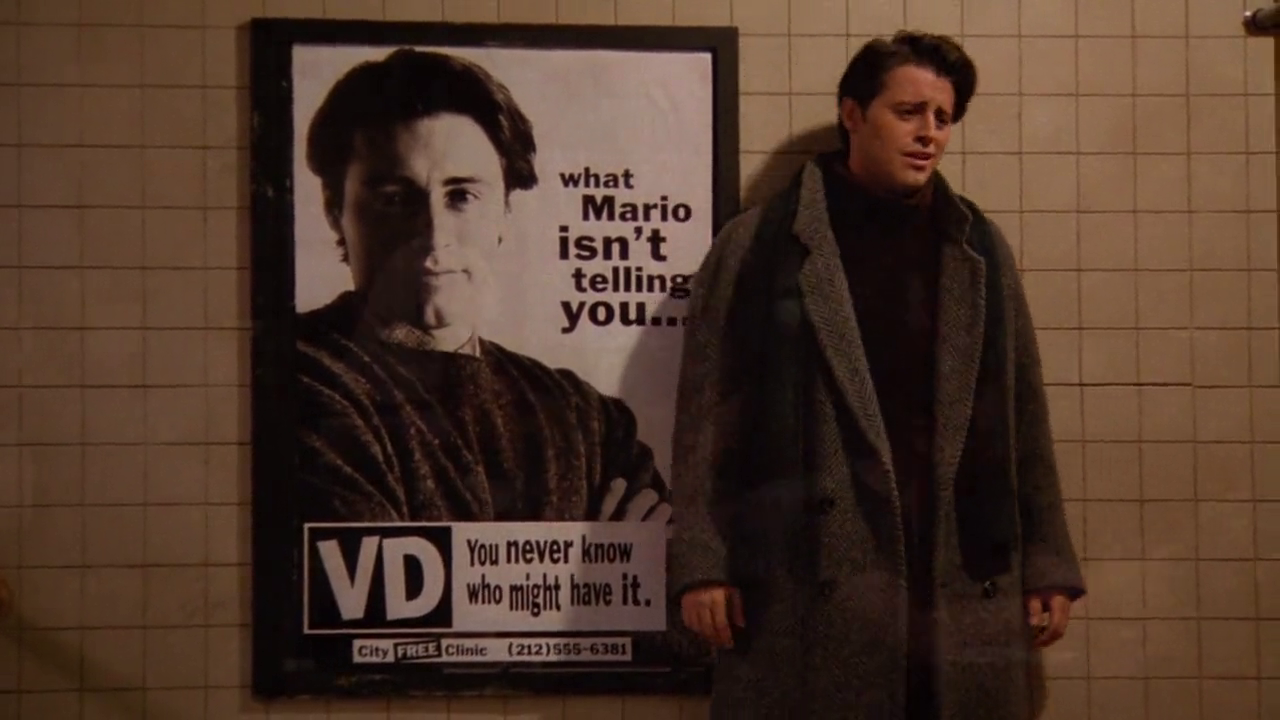
\includegraphics[trim={0 4cm 0 2cm,}, clip, width=\paperwidth]{./S01/img/9/dont-stand-so-close-to-me.png}
    \caption{Don’t Stand So Close To Me\label{fig:don-t-stand-so-close-to-me}}
  \end{adjustwidth}
\end{figure}

Após Joey descobrir que foi escolhido para o poster sobre VD (abreviação
de \emph{Venereal disease} ou Doença Venérea), é possível ouvir a música
\emph{Don't Stand So Close To Me} do álbum \emph{Zenyattà Mondatta}
(1980) da banda de rock britânica \emph{The Police}.

\begin{figure}
  \centering
  \begin{tikzpicture}
    \node [inner sep=0pt] at (0,0) {
      
\includegraphics[width=0.6\textwidth,keepaspectratio]{./S01/img/9/zenyatta-mondatta.jpg}
    };
    \draw [white, rounded corners=\ClipSep, line width=\ClipSep]
    (current bounding box.north west) --
    (current bounding box.north east) --
    (current bounding box.south east) --
    (current bounding box.south west) -- cycle
    ;
    \end{tikzpicture}
    \caption{Zenyattà Mondatta\label{fig:zenyatt-mondatta}}
\end{figure}

\emph{Sting}, o vocalista, é citado em
\textbf{\textcolor{primarycolor}{S01E13 - Aquele dos Seios}}, por Gloria
Tribbiani, mãe do Joey.

A banda é novamente citada no episódio
\textbf{\textcolor{primarycolor}{S08E10 - Aquele das botas da Monica}},
onde a Phoebe tenta conhecer o \emph{Sting} através do Ben, filho do
Ross.

\hypertarget{referuxeancias-2}{%
\subsection{Referências}\label{referuxeancias-2}}

\begin{itemize}
\tightlist
\item
  \sloppy Site oficial. \url{https://www.thepolice.com/zenyatta-mondatta}
\item
  \sloppy Vídeo clip - YouTube. \url{https://www.youtube.com/watch?v=KNIZofPB8ZM}
\end{itemize}

\hypertarget{a-very-special-blossom}{%
\section{A very special Blossom}\label{a-very-special-blossom}}

\begin{figure}[!ht]
  \begin{adjustwidth}{-\oddsidemargin-1in}{-\rightmargin}
    \centering
    
\includegraphics[trim={0 5cm 0 2cm,}, clip, width=\paperwidth]{./S01/img/9/blossom.png}
    \caption{Blossom\label{fig:blossom}}
  \end{adjustwidth}
\end{figure}

\begin{tcolorbox}[enhanced,center upper,
    drop fuzzy shadow southeast, boxrule=0.3pt,
    lower separated=false,
    colframe=black!30!dialogoBorder,colback=white]
\begin{minipage}[c]{0.14\linewidth}
  \raisebox{\dimexpr-\height+\ht\strutbox\relax}{
    
\includegraphics[width=1.5cm]{./assets/img/joey.png}
  }
   & \centering \scriptsize{Joey}
\end{minipage}
\hspace{.1mm}
\begin{minipage}[c]{0.8\linewidth}
  \textbf{- Set another place for Thanksgiving. My entire family thinks I have VD.}\\
  - Vou jantar aqui. Minha família acha que tenho doença venérea.
\end{minipage}

\medskip
\begin{minipage}[c]{0.14\linewidth}
  \raisebox{\dimexpr-\height+\ht\strutbox\relax}{
    
\includegraphics[width=1.5cm]{./assets/img/chandler.png}
  }
   & \centering \scriptsize{Chandler}
\end{minipage}
\hspace{.1mm}
\begin{minipage}[c]{0.8\linewidth}
  \textbf{- Tonight, on a very special Blossom.}\\
  - Esta noite, em um capítulo muito especial de Blossom.
\end{minipage}
\end{tcolorbox}

A fala de Chandler possui duas referências. Em uma temos a \emph{sitcom}
americana \emph{Blossom} (1991-1995), que conta a história de uma
garota, \emph{Blossom Russo}, interpretada por \emph{Mayim Bialik}, que
mora com dois irmãos e o pai solteiro. Na outra temos o termo \emph{on a
very special\ldots{}}, bastante usado por \emph{sitcoms} ou séries
dramáticas para indicar que o episódio tratará de assuntos controversos,
como por exemplo doenças venéreas.

Esse diálogo é relevante também quando leva-se em conta a carreira de
Matthew Perry. Ele participou de um episódio especial de \emph{Growing
Pains}, chamado \emph{Second Chance} (1989). No papel de Sandy ele
namorava Carol, uma das protagonistas da série. Com a relação se
tornando cada vez mais séria, eles decidem comemorar e acabam
exagerando. Mais tarde Carol descobre que Sandy se envolveu em um
acidente de carro e está gravemente ferido no hospital. Ao final, Sandy
acaba falecendo, mostrando que nem sempre temos segundas chances.

\begin{figure}
  \centering
  \begin{tikzpicture}
    \node [inner sep=0pt] at (0,0) {
      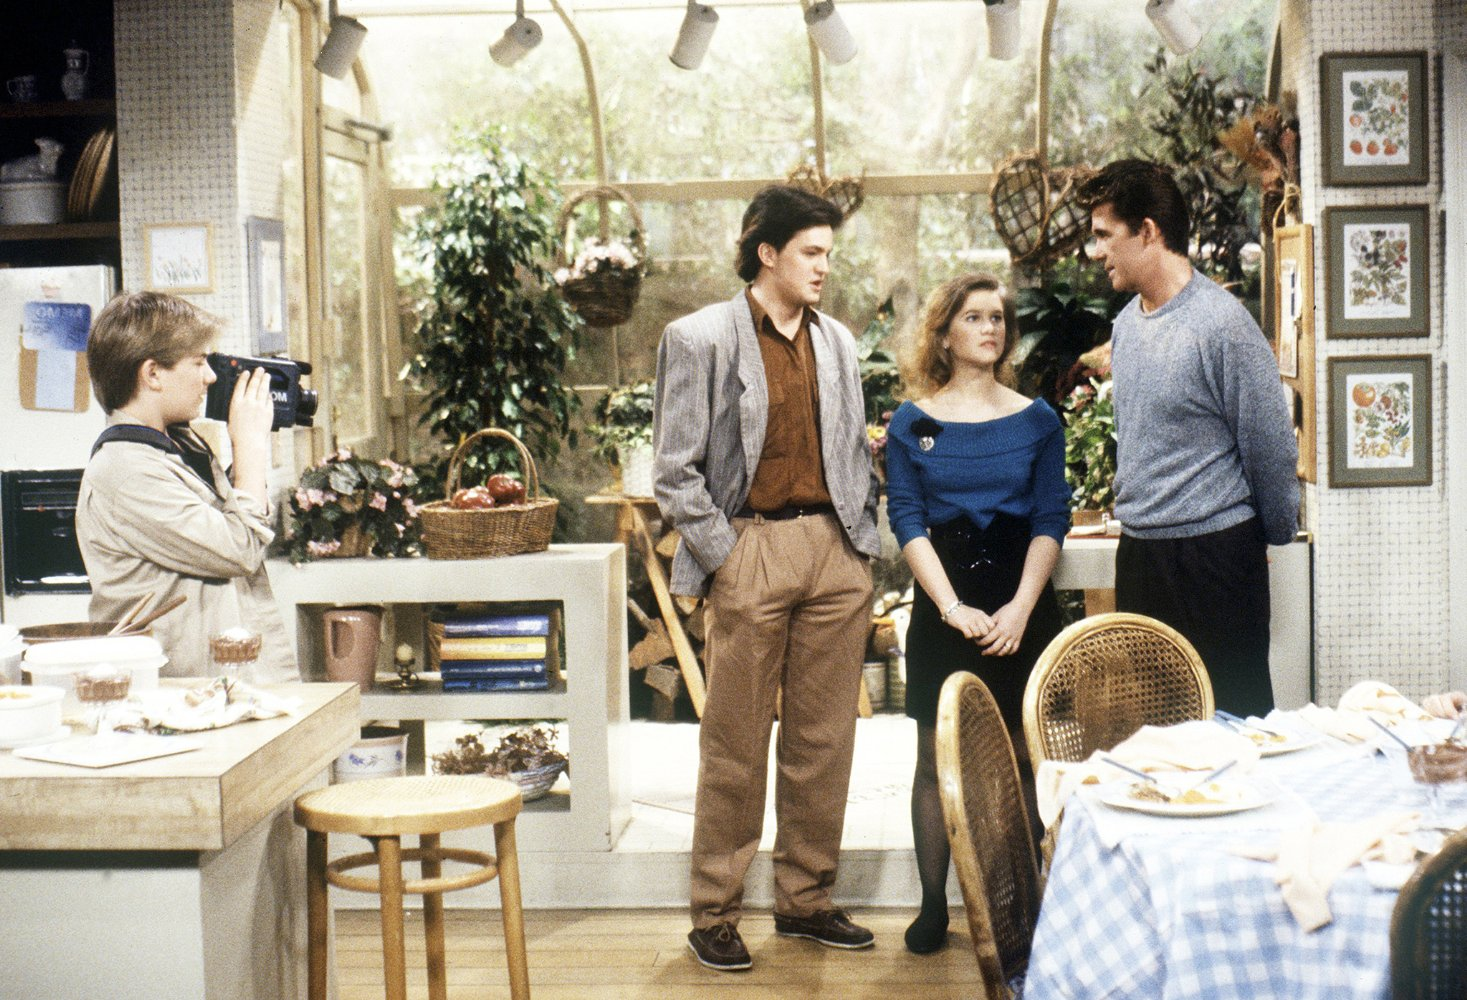
\includegraphics[width=0.8\textwidth,keepaspectratio]{./S01/img/9/growing-pains-second-chance.jpg}
    };
    \draw [white, rounded corners=\ClipSep, line width=\ClipSep]
    (current bounding box.north west) --
    (current bounding box.north east) --
    (current bounding box.south east) --
    (current bounding box.south west) -- cycle
    ;
    \end{tikzpicture}
    \caption{Cena de Second Chance - Growing Pains\label{fig:cena-de-second-chance-growing-pains}}
\end{figure}

\hypertarget{referuxeancias-3}{%
\subsection{Referências}\label{referuxeancias-3}}

\begin{itemize}
\tightlist
\item
  \sloppy Blossom - Fandom. \url{https://blossompedia.fandom.com/}
\item
  \sloppy Ep. Second Chance de Growing Pains - Fandom. \url{https://growing-pains.fandom.com/wiki/Second_Chance}
\item
  \sloppy Cenas de Matthew em Growing Pains - YouTube. \url{https://www.youtube.com/watch?v=o1nO-k1cw-w}
\item
  \sloppy Very especial episodes - Wikipédia. \url{https://en.wikipedia.org/wiki/Very_special_episode}
\item
  \sloppy Ep. The One Where Underdog Gets Away comentado - Genius. \url{https://genius.com/Friends-tv-the-one-where-underdog-gets-away-annotated}
\end{itemize}

\hypertarget{smokey}{%
\section{Smokey}\label{smokey}}

\begin{figure}[!ht]
  \begin{adjustwidth}{-\oddsidemargin-1in}{-\rightmargin}
    \centering
    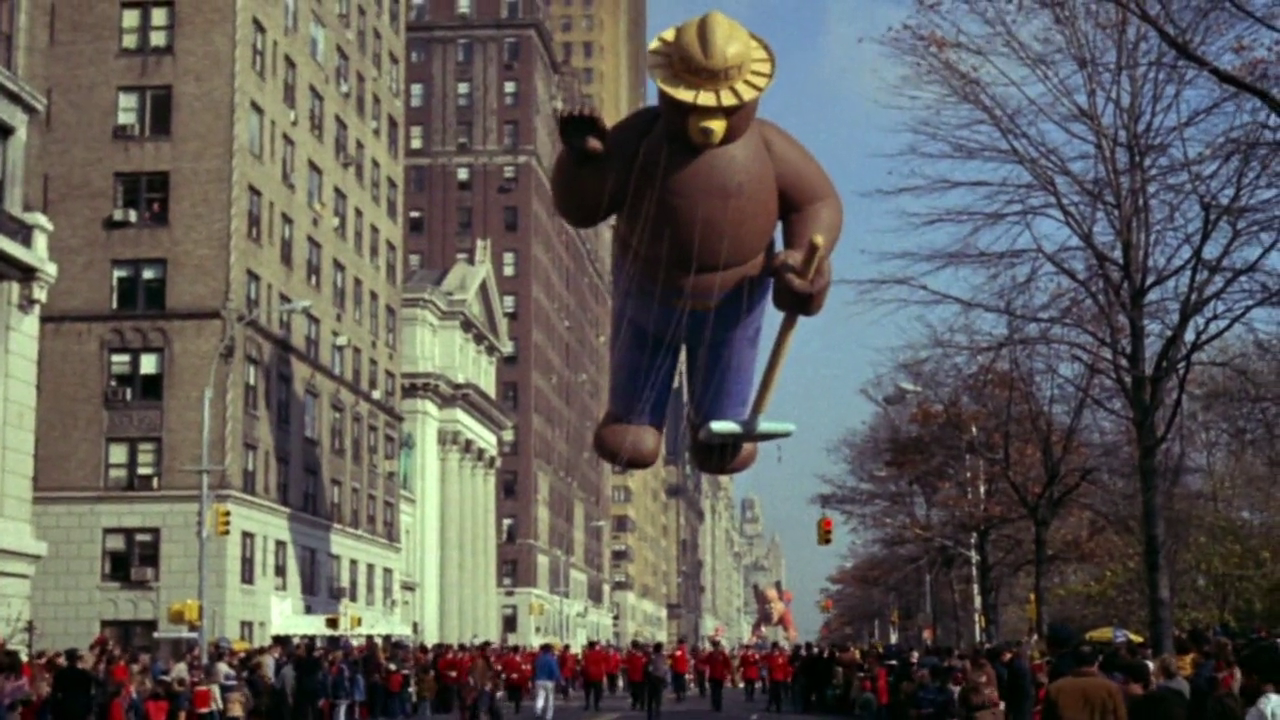
\includegraphics[trim={0 6cm 0 0cm,}, clip, width=\paperwidth]{./S01/img/9/smokey.png}
    \caption{Smokey\label{fig:smokey}}
  \end{adjustwidth}
\end{figure}

Enquanto os amigos assistem ao desfile de Ação de Graças, é possível ver
um balão inflado do urso \emph{Smokey} (1944), personagem criado para a
campanha de prevenção de incêndios florestais. Esse personagem é baseado
em um urso de verdade, que foi resgatado de uma floresta em chamas no
Novo México.

\hypertarget{referuxeancias-4}{%
\subsection{Referências}\label{referuxeancias-4}}

\begin{itemize}
\tightlist
\item
  \sloppy Site oficial. \url{https://www.smokeybear.com/en/smokeys-history/story-of-smokey}
\end{itemize}

\hypertarget{the-monkees}{%
\section{The Monkees}\label{the-monkees}}

\begin{figure}[!ht]
  \begin{adjustwidth}{-\oddsidemargin-1in}{-\rightmargin}
    \centering
    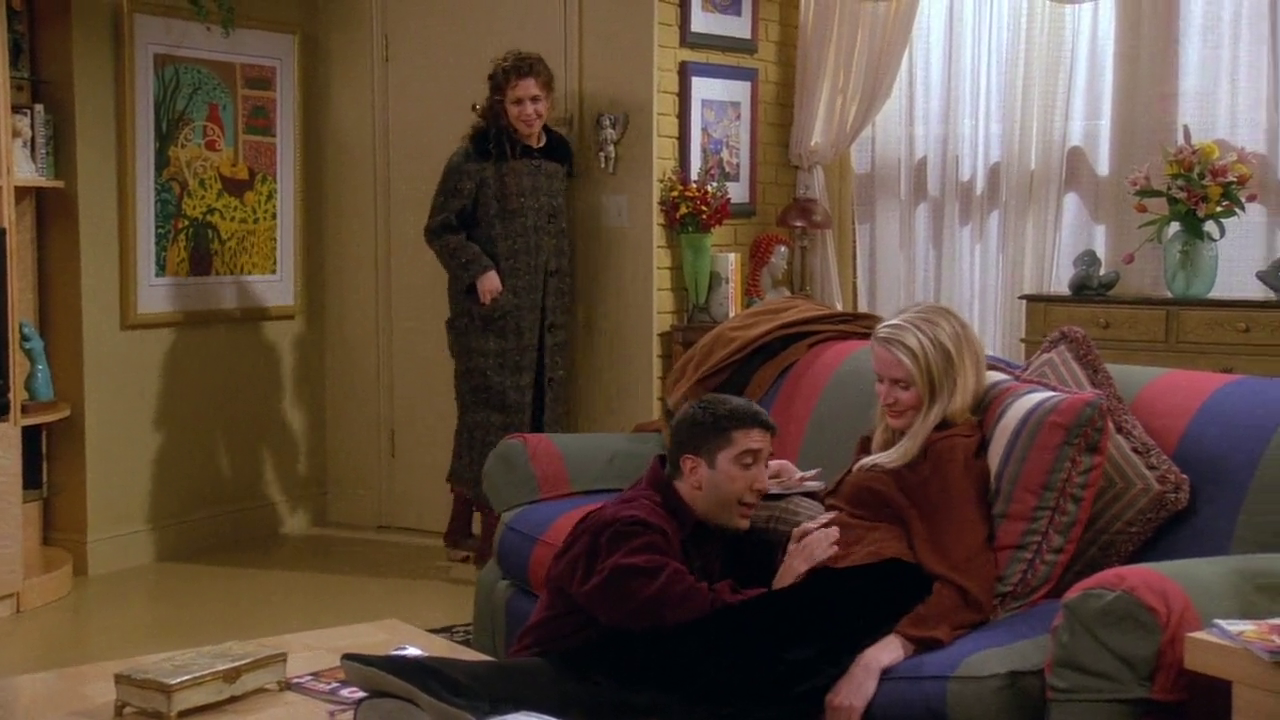
\includegraphics[trim={0 4cm 0 2cm,}, clip, width=\paperwidth]{./S01/img/9/the-monkees.png}
    \caption{The Monkees\label{fig:the-monkees}}
  \end{adjustwidth}
\end{figure}

Quando finalmente decide cantar para o bebê ainda na barriga de Carol,
Ross escolhe a canção \emph{(Theme From) The Monkees} (1966) da série de
comédia americana \emph{The Monkees}. Ross canta o primeiro trecho
corretamente, mas depois, notavelmente, inventa o restante. Confira o
trecho cantado corretamente:

\bigskip
\begin{tcolorbox}[enhanced,
    drop fuzzy shadow southeast, boxrule=0.3pt,
    lower separated=false, sidebyside, sidebyside align=top,
    halign=flush right, halign lower=left,
    colframe=black!30!dialogoBorder,colback=musicaBg]
\includegraphics[width=0.4cm]{./assets/img/icon-music.png}\\
Here we come\\Walkin’ down the street\\We get the funniest looks from\\Everyone we meet\\
\tcblower
\includegraphics[width=0.4cm]{./assets/img/icon-language.png}\\
Aqui vamos nós\\Andando rua abaixo\\Nós conseguimos os olhares engraçados de\\Cada um que nós conhecemos\\
\end{tcolorbox}

\begin{figure}
  \centering
  \begin{tikzpicture}
    \node [inner sep=0pt] at (0,0) {
      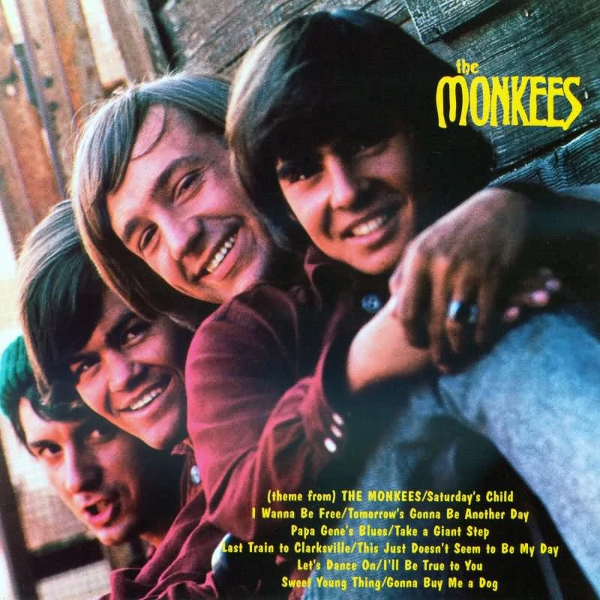
\includegraphics[width=0.6\textwidth,keepaspectratio]{./S01/img/9/the-monkees-poster.png}
    };
    \draw [white, rounded corners=\ClipSep, line width=\ClipSep]
    (current bounding box.north west) --
    (current bounding box.north east) --
    (current bounding box.south east) --
    (current bounding box.south west) -- cycle
    ;
    \end{tikzpicture}
    \caption{The Monkees poster\label{fig:the-monkees-poster}}
\end{figure}

\hypertarget{referuxeancias-5}{%
\subsection{Referências}\label{referuxeancias-5}}

\begin{itemize}
\tightlist
\item
  \sloppy Fandom - Wiki. \url{https://monkees.fandom.com/wiki/Monkeepedia}
\item
  \sloppy Tema de abertura - YouTube. \url{https://www.youtube.com/watch?v=96A0uyFWQHs}
\end{itemize}
